%!TEX root = GRoutes.tex
%%%%%%%%%%%%%%%%%%%%%%%%%%%%%%%%%%%%%%%%%%%%%%%%%%%%%%%%%%%%%%%%%%%%%%%
\chapter{GRoutes - alkalmazás bemutatása}\label{ch:ALAP}
%%%%%%%%%%%%%%%%%%%%%%%%%%%%%%%%%%%%%%%%%%%%%%%%%%%%%%%%%%%%%%%%%%%%%%%

\begin{osszefoglal}
	Ebben a fejezetben a GRoutes android applikációt fogom bemutatni úgy technikai, mint funkcionális szempontból.
	
\end{osszefoglal}

%%%%%%%%%%%%%%%%%%%%%%%%%%%%%%%%%%%%%%%%%%%%%%%%%%%%%%%%%%%%%%%%%%%%%%%
\section{Funkcionalitások}\label{sec:ALAP:adatelem}

\subsection{Bejelentkezés}

\begin{wrapfigure}{l}{0.4\linewidth}
	\centering
	\setlength{\abovecaptionskip}{0pt}
	\setlength{\belowcaptionskip}{0pt}
	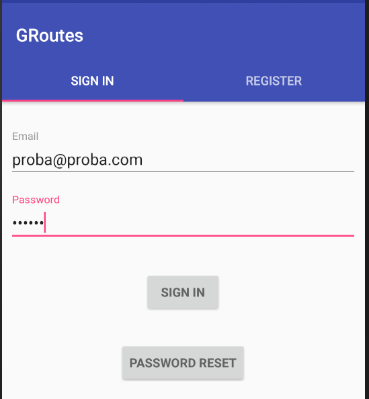
\includegraphics[width=0.4\textwidth]{images/login}
	\caption{Bejelentkezési felület\label{fig:ALAP:sm2}}
\end{wrapfigure}

Az alkalmazás elindítása után egy bejelentkezési felület fogadja a felhasználót. Itt kell megadni az e-mail címet, valamint a jelszót amivel a felhasználó regisztrált. Amennyiben elfelejtette a jelszavát, az "elfelejtett jelszó" gomb megnyomásával lehetőség van egy jelszó-visszaállító e-mail kiküldésére. 

Ha egy új felhasználó szeretné igénybe venni az applikáció szolgáltatásait, akkor regisztrálnia kell. Ezt megteheti a regisztráció lapra való navigálás után, melyet a cím megérintésével, vagy a képernyőn az ujjának balra történő húzásával érheti el. Az e-mail cím és az új jelszó megadása után, a felhasználó egyből a főmenübe érkezik, mindeközben azonban egy aktivációs e-mailt is kap arra a címére, amivel regisztrált. A későbbiekben csak akkor fog tudni bejelentkezni, ha a kapott emailben az URL%
\footnote{ %
	Uniform Resource Locator, más néven webcím
}  %
-re klikkelve aktiválja a felhasználóját.

\subsection{Főmenü}

A főmenüből négy különböző oldalra navigálhatunk tovább: a keresési felület, a régebbi keresések megtekintése, a kedvencek menedzselése, valamint a beállítások. Az ötödik (csoportok) oldal egy jövőbeli funkcionalitás kifejlesztésére van fenntartva.

\subsection{Keresési felület}

Ezen a felületen van lehetőségünk útvonalak, helyszínek keresésére. Az "+" gomb megjelnít egy új mezőt, ahol további címeket adhatunk meg. A "nagyító" gomb a térkép felületre navigál, és kirajzolja a tervezett útvonalat. A keresés elindítása előtt, minden cím mellett van egy "térkép" gomb, ennek segítségével tudjuk megnézni, hogy valóban az az a hely, amire gondoltunk.

\subsection{Kedvencek}
 
 Itt jelennek meg az általunk manuálisan elmentett utak, helyszínek. Minden bejegyzésnél négy gomb jelenik meg, ezeknek az funkcióik a következők:
 
 \begin{description}
 	\setlength{\itemsep}{0.04mm}
 	\item[térkép] -- megjeleníti a térkép felületet, ahol ráközelít a helyszín koordinátáira, vagy kirajzolja az útvonalat.
 	\item[nagyító] -- a keresési felülethez navigál és kitölti a keresési mezőket, az útvonal csomópontjaíval, így a felhasználó könnyedén módosíthatja útvonaltervét.
 	\item[ceruza] -- módosítja a bejegyzés nevét.
 	\item[szemetes veder] -- törli a bejegyzést, ezáltal az adatbázisból is törlődni fog.
 \end{description}

\subsection{Múltbeli keresések}

A keresési felület eredményéül kapott útvonalak megjelennek a múltbeli keresések menüpont alatt, nevüket a keresési dátum és időpont alkotja. A bejegyzéseknél a "Kedvenceknél" tárgyalt gombok találhatóak, azonos funkcióval, azzal a kivétellel, hogy a "ceruza" gombot a "csillag" helyettesíti, melynek segítségével elmenthetünk egy útvonalat a kedvencek közé.

\subsection{Beállítások}

Itt ki tudjuk választani a limitet, hogy mennyi csomópont esetén, melyik algoritmust használja az alkalmazás. A megadott számnál kisebb vagy egyenlő számú csomópontok esetén a \(Concorde\) nevű egzakt megoldásokat nyújtó algoritmus fogja kiszámolni az ideális útvonalat. Ez az algoritmus a legpontosabb megoldásokat nyújtja, azonban az "utazó ügynök" problémájának komplexitása miatt, a csomópontok növekedésével, a végrehajtási idő is exponenciálisan növekszik. Amennyiben a felhasználó nagyon sok csomóponttal szeretne dolgozni, és fontosabb neki az, hogy belátható időn belül egy elfogadható megoldást kapjon, de nem probléma, ha nem a leghatékonyabb útvonal rajzolódik ki, akkor a megadott szám feletti mennyiségű csomópontok esetén, az applikáció egy úgynevezett \(greedy\)%
\footnote{ %
	mohó
}  %
 algoritmust fog használni. Ez nagyságrendekkel gyorsabb az exponenciálishoz viszonyítva, azonban nem minden esetben nyújtja a legjobb megoldást.

Ugyanitt megadhatjuk az alapértelmezett utazási módot, ami lehet gyaloglás, valamint vezetés.

Bár az egyszerűség kedvéért igyekeztem sok írás helyett szimbólumokat tenni a gombokra, de az applikációban található kevés szövegnek a nyelvét szintén itt lehet beállítani.

A térképpel, navigációval kapcsolatos paraméterek módosítására is van lehetőség, mint példaul az alapértelmezett nagyítás, a pozíció lekérésének gyakorisága, a térképre való automatikus ránagyítás és ennek centralizálásának a gyakorisága navigáció közben, valamint a megtett út kirajzolásának a mennyisége.

\subsection{Térkép felület}

Ez a felület akkor jelenik meg, amikor megérintjük a térkép gombot egy helyszín vagy egy útvonal mellett, valamint a keresési felület eredménye is itt rajzolódik ki.
Amennyiben egy helyszíntől érkezünk, megjelenik egy \(marker\)%
\footnote{ %
	jelző
}  %
az adott koordinátán.

A "csillag" gomb segítségével hozzáadhatunk egy helyszínt vagy egy útvonalat a kedvencekhez, ahol később visszanézhetjük, módosíthatjuk a nevét. Alapértelmezetten, a bejegyzések neve a keresési dátum és időpont lesz. A "nagyító" gomb segítségével visszatérhetünk a keresési felületre, így könnyedén módosíthatjuk tervezett útvonalunkat. Az "navigáció" gomb segítségével elkezdhetünk navigálni a tervezett útvonalon.

%%%%%%%%%%%%%%%%%%%%%%%%%%%%%%%%%%%%%%%%%%%%%%%%%%%%%%%%%%%%%%%%%%%%%%%
\section{Adatbázis}\label{sec:ALAP:adatelem}

 \begin{wrapfigure}{l}{0.5\linewidth}
	\centering
	\setlength{\abovecaptionskip}{0pt}
	\setlength{\belowcaptionskip}{0pt}
	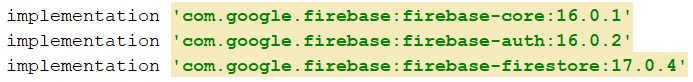
\includegraphics[width=0.5\textwidth]{images/firebase_gradle}
	\caption{A Firebase függőségei\label{fig:ALAP:sm2}}
\end{wrapfigure}

Adatbázisnak és az autentikáció menedzselésére Firebase-t használtam. Mielőtt bármilyen funkcióját is használhatnám ennek az applikációfejlesztési platformnak, be kellett jelentkezzek a Google felhasználómmal, csinálnom kellett egy projektet, majd ezt a projektet össze kellett kapcsolnom magával az applikációval amit fejleszteni szerettem volna. Van egy külön \(plugin\)%
\footnote{ %
	kiegészítés
}  %
 az \(Android Studio\)%
 \footnote{ %
 	fejlesztési környezet android applikációk számára
 }  %
-ban, melynek segítségével könnyedén létre lehet hozni a ezt kapcsolatot. Előtte azonban az applikáció Gradle állományába be kellett jelentsem a \(core\), \(auth\) és \(firestore\) modulokat, mint függőségeket.
 

 

\subsection{Autentikáció}

A web-es felületen engedélyeznem kellett az e-mail/jelszó bejelentkezést. Ugyanitt állítottam be, hogy biztonsági okokból maximum hány regisztrációt engedjen a rendszer óránként ugyanarról az IP címről, jelenleg ez 100. Regisztációkor generálódik egy egyedi felhasználói ID, ennek segítségével oldom meg, hogy minden felhasználó csak a saját adataihoz férjen hozzá. A bejelentkezés, regisztráció, jelszó visszaállító e-mail küldése műveleteket a FirebaseAuth \(singleton\)%
\footnote{ %
	egy tervezési minta, az adott osztályból egy és csak is egy objektumot lehet létrehozni
}  %
 osztály metódusaival oldottam meg.
 
 \begin{description}
 	\setlength{\itemsep}{0.04mm}
 	\item[createUserWithEmailAndPassword(email, jelszó)] -- kreál egy felhasználót az e-mail és jelszó karakterlánc paraméterek segítségével, majd sikeres válasz után be is jelentkezik
 	\item[signInWithEmailAndPassword(email, jelszó)] -- megpróbál bejelentkezni a megadott e-mail/jelszó kombinációval
 	\item[sendPasswordResetEmail(email)] -- küld egy jelszó visszaállító e-mailt a paraméterként megadott címre.
 \end{description}

Az aktiváviós e-mail küldéséhez a FirebaseUser osztály insztanciájának a sendEmailVerification() metódusát használtam.

\subsection{Kollekciók, Dokumentumok}

\begin{wrapfigure}{l}{0.6\linewidth}
	\centering
	\setlength{\abovecaptionskip}{0pt}
	\setlength{\belowcaptionskip}{0pt}
	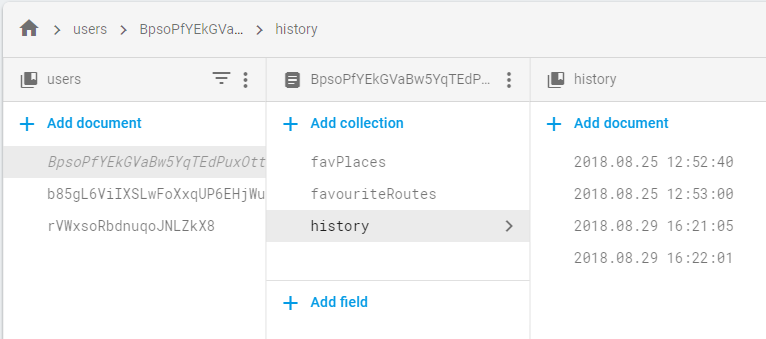
\includegraphics[width=0.6\textwidth]{images/firestore_colls}
	\caption{Firestore kollekciók\label{fig:ALAP:sm2}}
\end{wrapfigure}

A Firestore egy még Beta%
\footnote{ %
	még tesztelés alatt van
}  %
 verzióban levő no-sql, kulcs-érték párokra alapuló adatbázis, mely a Firebase platformon érhető el. Építőelemei a kollekciók és a dokumentumok, ezek váltakozva követik egymást, mivel egy kollekció csak dokumentumokat tartalmazhat, egy dokumentom viszont a kollekciók mellett adatokat (kulcs-érték párok) is tartalmazhat. 
 
 \begin{wrapfigure}{l}{0.6\textwidth}
 	\centering
 	\setlength{\abovecaptionskip}{0pt}
 	\setlength{\belowcaptionskip}{0pt}
 	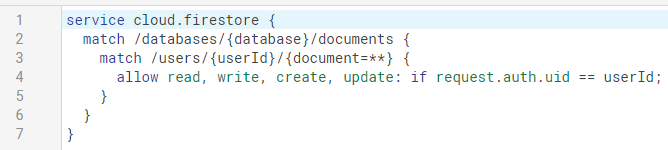
\includegraphics[width=0.6\textwidth]{images/firestore_rule}
 	\caption{Firestore szabály\label{fig:ALAP:sm2}}
 \end{wrapfigure}
 
Minden felhasználónak csak a saját dokumentumához van hozzáférése. Ezt egy úgynevezett szabály meghatározásával lehet elérni. Az adatbázis minden beérkező függvényhívást kiértékel a szabály alapján, és eldönti, hogy az adott kérésnek van-e elegendő jogosultsága. Amennyiben nincs, csak egy hibaüzenetet térít vissza.

 A GRoutes alkalmazás esetében a következőképpen építettem fel a struktúrát: vagy egy \(users\) kollekció, amely a felhasználókat tartalmazza. Minden felhasználói dokumentumnak az ID-ja megegyezik az UID%
\footnote{ %
	egyedi felhasználói ID, ami regisztrációkor generálódik
}  %
-val. A felhasználói dokumentumok a \(favPlaces\), \(favouriteRoutes\) és \(history\) kollekciókat tartalmazzák, melyek rendre megfelelnek a "kedvenc helyek", "kedvenc útvonalak" és "múltbeli útvonalak" fogalmaknak. Ezek a kollekciók tartalmazzák a különböző bejegyzéseknek (helyek, útvonalak) megfelelő dokumentumokat, melyek magukat az adatokat tartalmazzák. Az adatok sajátos entitás objektumok, melyeket a kódban, bizonyos szabályok alapján, de az én elképzelésem szerint hoztam létre. 


Egy út tartalmaz egy hely objektumokból álló tömböt a csomópontok számontartására, egy indexekből álló tömböt a csomópontok sorrendjének tárolására, valamint egy név mezőt.

Egy hely objektum tartalmaz egy-egy karakterlánc típusú név és cím mezőt, valamint egy GeoPoint objektumot, ami a hely főldrajzi szélességi és hosszúsági fokait tárolja.
 

%%%%%%%%%%%%%%%%%%%%%%%%%%%%%%%%%%%%%%%%%%%%%%%%%%%%%%%%%%%%%%%%%%%%%%%
\section{Osztályok}\label{sec:ALAP:adatelem}

\subsection{Activity-k}\label{sec:ALAP:adatelem}

\subsection{Assist osztályok}\label{sec:ALAP:adatelem}

\subsection{Általános segédosztályok}\label{sec:ALAP:adatelem}

\subsection{Entitás osztályok}\label{sec:ALAP:adatelem}

\begin{figure}
	\centering
	\setlength{\abovecaptionskip}{0pt}
	\setlength{\belowcaptionskip}{0pt}
	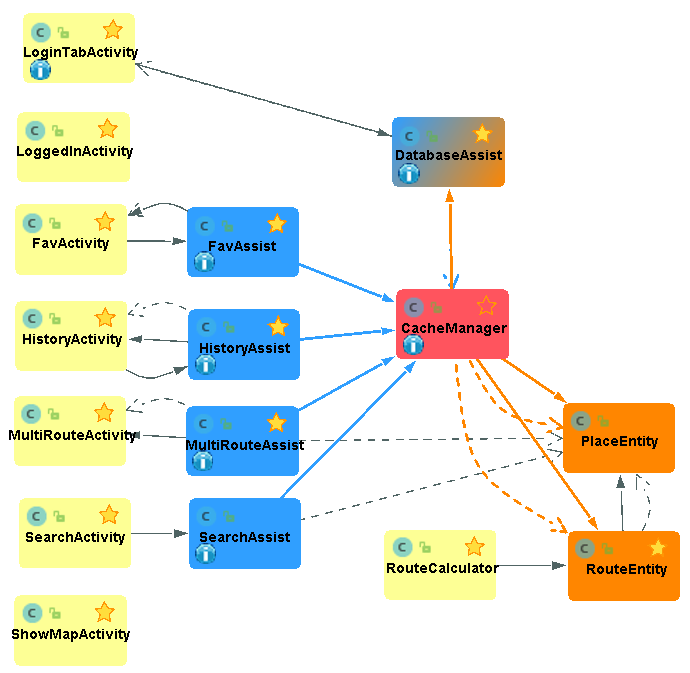
\includegraphics[width=0.6\textwidth]{images/class_diagram}
	\caption{Osztálydiagramm\label{fig:ALAP:sm2}}
\end{figure}

%%%%%%%%%%%%%%%%%%%%%%%%%%%%%%%%%%%%%%%%%%%%%%%%%%%%%%%%%%%%%%%%%%%%%%%
\section{Felmerülő problémák}\label{sec:ALAP:adatelem}

